This chapter gives an overview of the fundamental concepts and the algorithms important for this thesis.

\section{Machine Learning}\label{background:machine_learning}

Machine Learning is a sub-field of Artificial Intelligence that builds models based on statistical and algorithmic concepts in order to detect relevant patterns based on previously-seen data \cite{geron_2019}. There are four categories of learning, i.e., \textit{supervised}, \textit{semi-supervised}, \textit{unsupervised} and \textit{reinforcement learning} \cite{Sarker2021}. Each category performs different types of tasks on different types of data. This study focuses only on supervised learning.

In supervised learning, algorithms build mathematical models from labeled data, which is data in the format $(X, y)$, where $X$ is the input sample and $y$ is the expected output, or label. During training, algorithms provide the model with the input samples and improve the model by comparing its output with the expected outputs (the so called ground truth). Supervised learning problems can be divided into \textit{regression problems}, if the output is a continuous variable, or \textit{classification problems}, if the output is a discreet variable \cite{Sarker2021}.

\subsection{Federated Learning}\label{background:federated_learning}

Federated Learning is a ML technique, in which different distributed clients collaboratively train a model under the supervision of a centralized server. Clients are distributed heterogeneous devices with their own computing resources and they are responsible for producing and maintaining their own data \cite{9084352}. The data is assumed to be non independent or non identically distributed (\textit{non-iid}).

Since clients are heterogeneous and distributed, having different communication costs and response times are normal. In addition, some clients may operate under constrained networks with either low or limited bandwidth. Therefore, it is important that new FL techniques ensure that communication and resource usage is minimized.

During the training process, the raw data never leaves the clients and only the model parameters, such as model weights, are exchanged with the server in order to compute the global model. However, model weights can be target of inference attacks and leak secret information \cite{10.1145/3298981}.  Consequently, new Federated Learning architectures and algorithms must be compatible with techniques that guarantee privacy, such as differential privacy, homomorphic encryption, secure multiparty computation or other cryptographic protocols \cite{10.1145/3298981}.

After each round of training, the central server aggregates the local updates. Usually, this is done using a mathematical formula, for example, Federated Averaging (\textit{FedAvg}) \cite{10.48550/arxiv.1602.05629}, which calculates the weighted average of all clients.
% $k \in K$ weights $w^k$:

% \begin{equation}
% w_{t+1} = \sum_{k \in K} \frac{n_k}{n} w_{t+1}^k
% \end{equation} \label{eq:fedavg}

% Where $n_k$ is the number of samples that the client $k$ used to train and $w_{t+1}^k$ the weights of client $k$ at round $t+1$.

\subsection{Categories of Federated Learning}\label{background:archfl}

According to \cite{10.1145/3298981, 10.1145/3412357}, with respect to the different data partition among the clients, the federated Learning techniques can be broadly divided into three main categories, i.e., (i) 
horizontal, (ii) vertical, and (iii) federated Transfer Learning. We focus on the first two categories.

In \textit{Horizontal Federated Learning} (HFL), clients with the same data structure collaborate to build a single model. In other words, the different data sets in the different clients share the same feature space, but not the sample space. For example, two banks branches operating in different cities have similar businesses (feature space), but different clients (sample space). The architecture of HFL, depicted in \autoref{fig:hfl_arch}, consists of multiple clients training a model, while the central server performs the aggregation of all local updates.

In \textit{Vertical Federated Learning} (VFL), clients share an intersecting sample space, but different feature spaces. For example, two different banks with different products operating in the same city have a similar client base (sample space), but different information about each client (feature space). The architecture of VFL, depicted in \autoref{fig:vfl_arch}, is similar to the one of HFL. However, it requires an additional step, calculating the Private Set Intersection (PSI) \cite{wei2022vertical}, since the clients do not share the exact same sample space. PSI is a protocol by which multiple clients can calculate the common samples without sharing their raw data \cite{wei2022vertical}.

\begin{figure}[!htp]
    \centering
    \centering
    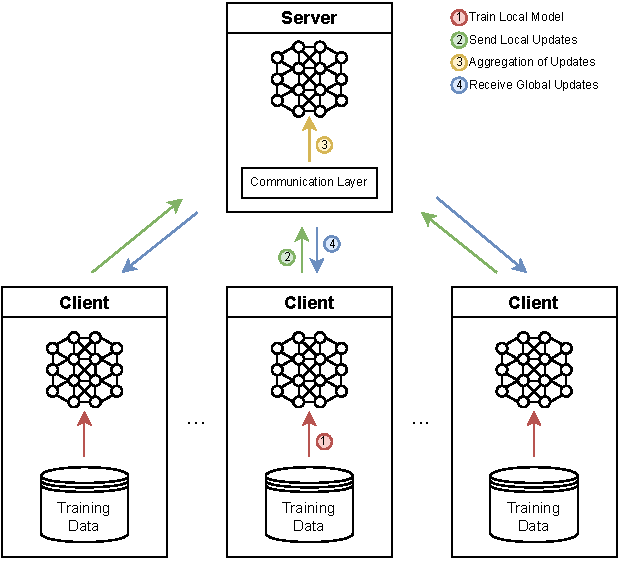
\includegraphics[width=0.6\textwidth]{graphics/hfl-architecture.pdf}
    \caption{Horizontal Federated Learning Architecture}
    \label{fig:hfl_arch}
\end{figure}

\begin{figure}[!hbp]
    \centering
    \centering
    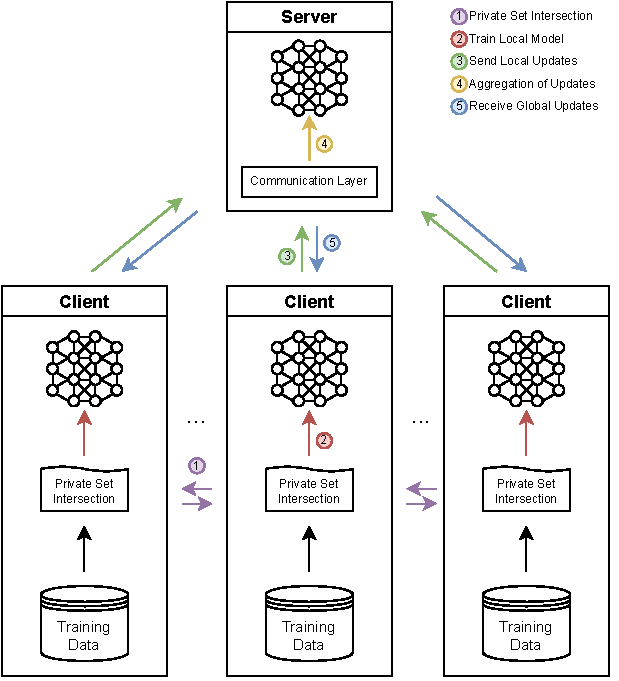
\includegraphics[width=0.6\textwidth]{graphics/vfl-architecture.pdf}
    \caption{Vertical Federated Learning Architecture}
    \label{fig:vfl_arch}
\end{figure}

\section{Blockchain}\label{background:blockchain}

A blockchain is an immutable distributed ledger, which is a database of transactions maintained by several computers, also known as nodes, linked through a peer-to-peer network. The concept of blockchain was first introduced by Stuart Haber and W. Scott Stornetta in 1991 \cite{10.48550/ARXIV.1810.06130}, being popularized by Satoshi Nakamoto in 2008 with the introduction of the cryptocurrency Bitcoin \cite{nakamoto2009bitcoin}.

\begin{figure}[h]
    \centering
    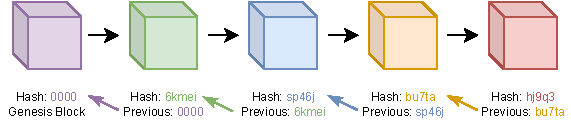
\includegraphics[width=0.8\textwidth]{graphics/blockchain.pdf}
    \caption{Blockchain Representation}
    \label{fig:blockchain_blocks}
\end{figure}

In a blockchain, the data is structured as blocks, as can be seen in \autoref{fig:blockchain_blocks}. Each block contains a certain number of transactions and links to the previous block via a cryptographic hash, forming a chain. This guarantees fidelity and trust without requiring a trusted third party, which is why it is called a \textit{trustless} system. In addition, since the record is immutable and decentralized, all transactions can be transparently viewed by others.

As mentioned beforehand, a blockchain is maintained by several nodes in a peer-to-peer network. As transactions come in, nodes compete in order to generate the next block. Since it is a decentralized process, multiple nodes will try to create the next block of the chain in parallel. In order to reach an agreement between the nodes, a consensus algorithm is used. The consensus algorithm allows to reach an agreement between multiple decentralized nodes without requiring a singular node to be in charge.

\begin{figure}[h]
    \centering
    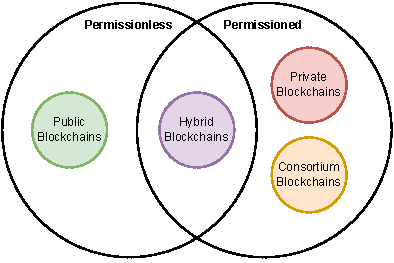
\includegraphics[width=0.5\textwidth]{graphics/blockchain-types.pdf}
    \caption{Blockchain Types}
    \label{fig:blockchain_types}
\end{figure}

\autoref{fig:blockchain_types} illustrates four different types of blockchain, i.e., public, private, consortium, and hybrid. Some are permissionless, which means that anyone can join the network, while some are permissioned, which means that only allowed parties can join the network. 

\begin{itemize}
    \item \textit{Public Blockchains} are permissionless and therefore anyone can join and participate in the network. There is no central authority.

    \item \textit{Private Blockchains}, in contrary to the public blockchains, private blockchains are permissioned with a single central authority. They can only be accessed by allowed parties and they are usually used within organizations.

    \item \textit{Consortium Blockchains}, similarly to the private blockchains, are permissioned. However, instead of being controlled by a single authority, they are controlled by a group of different authorities.

    \item \textit{Hybrid Blockchains} have features of both permissioned and permissionless blockchain systems. They, on one hand, are usually controlled by a single authority, while on the other hand, have a mixed usage of permissioned and permissionless protocols running in parallel for different use cases.
\end{itemize}

\subsection{Smart Contracts}\label{background:smart_contracts}

Smart contracts \cite{8500488} are small computer programs that live within the blockchain and automatically run when predetermined conditions are met. As they live in the blockchain, they are trustless and are typically used to automate the execution of agreements. This way, every party involved in the agreement is certain that it will be honored once the conditions of the agreement are met. Some blockchain platforms, such as the Ethereum \cite{wood2014ethereum}, provide functionality for smart contracts.

\subsection{Blockchain Platforms}\label{background:blockchain_platforms}
 
As explained in \autoref{background:blockchain}, blockchain platforms allow developers to build applications on top of the blockchain technologies. Even though all platforms are based on the concept of blockchain, they all have different characteristics and restrictions, as well as different sets of features.

As it can be seen in \autoref{tab:platf_consensus}, around half of the implementations used an already existing platform, where the remaining preferred to implement their own blockchain platform. Among already existing platforms, Ethereum is the most popular. When implementing a custom platform, it is easier to overcome certain restrictions such as limits on data per block \cite{8733825, 9524833}.

\subsection{Consensus Algorithm}\label{background:consensus_algorithms}

The consensus algorithm is one of the most important components of a Blockchain platform. Consensus is the process of reaching an agreement on a single value among different distributed processes \cite{9347812}. These algorithms are designed to be reliable even on networks that have unreliable blockchain nodes. In blockchain, the consensus algorithm is used to reach consensus on the next block of the chain \cite{9079513}. The following consensus algorithms will be compared in our work:

\begin{itemize}
    \item The \textit{Proof of Work (PoW)} \cite{finney} consensus algorithm was first introduced in the context of blockchain platforms by Satoshi Nakamoto in Bitcoin \cite{nakamoto2009bitcoin}. It works by means of computation effort proofs, where a set of virtual miners race in solving a complex, yet feasible, mathematical problem. The winner of the race generates a cryptographic proof based on the solution of the problem that can be easily verified by others. Then, the winner adds a new block containing the newly verified transactions to the blockchain. In addition, the winner is rewarded according to some pre-determined rules.
    
    On the one hand, it is a simple algorithm, for which proofs are hard to create, but easy to verify \cite{li_blockchain_2021}. Not only is it robust and proven to work, but the cost of attacking a PoW blockchain is extremely high \cite{li_blockchain_2021}. For an attack to be successful, it needs to control more than half of the network \cite{li_blockchain_2021}. On the other hand, PoW consumes extreme amounts of energy and it is hard to scale \cite{edwood_2020, li_blockchain_2021, ccaf}.
    
    \item The \textit{Proof of Authority (PoA)} \cite{szilagyi_2017} consensus algorithm is a reputation-based consensus algorithm that is most commonly used in private blockchain networks. It works by having a set of validator nodes that are responsible for validating new transactions. In order to ensure the correctness of the validator nodes, they have to stake their own reputation. In addition, the validators are known trusted entities that are manually chosen by the network owner.
    
    On the one hand, PoA provides high throughput and high scalability \cite{bPoA}. On the other hand, the main criticism of PoA is that it is usually has a small number of validators, that are manually chosen. Therefore, it has a lesser degree of decentralization. Consequently, PoA is not as common in public blockchain networks as it is for private networks \cite{bPoA}.

    \item The \textit{QBFT Byzantine Fault Tolerance (QBFT)} \cite{10.48550/arxiv.2002.03613} consensus algorithm is similar to the Practical Byzantine Fault Tolerance (PBFT) \cite{Castro99practicalbyzantine} algorithm, which is a three-phase protocol that allows a network with $3f+1$ nodes, where $f$ is the maximum amount of faulty nodes, to reach consensus. The different between QBFT and PBFT is that in the former the set of validators is dynamic, while in the latter, it is static. The network reaches a consensus once $2f+1$ nodes agree.
    
    One the one hand, QBFT allows for high consensus efficiency in high throughput networks \cite{li_blockchain_2021}. On the other hand, it will stop working properly if only 33\% or less blockchain nodes are running and it can also have high communication costs due to its three-phase protocol nature \cite{li_blockchain_2021}.
\end{itemize}

\section{Blockchain-based Federated Learning}\label{background:bfl}

Recently, the idea of applying blockchain to FL has emerged. This is motivated by the fact that FL architectures are highly dependent on a single central server, leading to a central point of failure, that can be either overloaded or compromised. With blockchain, the central server can be replaced by multiple decentralized servers that operate the blockchain nodes. In addition, blockchain can provide authentication, traceability, auditability and data preservation.

As stated in \cite{10.48550/arxiv.2110.02182}, so far three different main architecture groups have been proposed for BFL systems: \textit{Fully Coupled BFL}, \textit{Flexibly Coupled BFL}, and \textit{Loosely Coupled BFL}. In Fully Coupled BFL, the distributed clients are the only devices in the network and act as both clients and servers, performing the training and aggregation, as well as running the blockchain nodes. In Loosely Coupled BFL, the central server still exists and blockchain is only used to manage the reputation of clients. Flexibly Coupled BFL provides a middle ground between both, where there are servers and clients in the network. The servers are responsible for maintaining the blockchain nodes and use the blockchain to store information such as aggregations, scores, among others. The architecture is depicted in \autoref{fig:bfl_arch}.

\begin{figure}[!ht]
    \centering
    \centering
    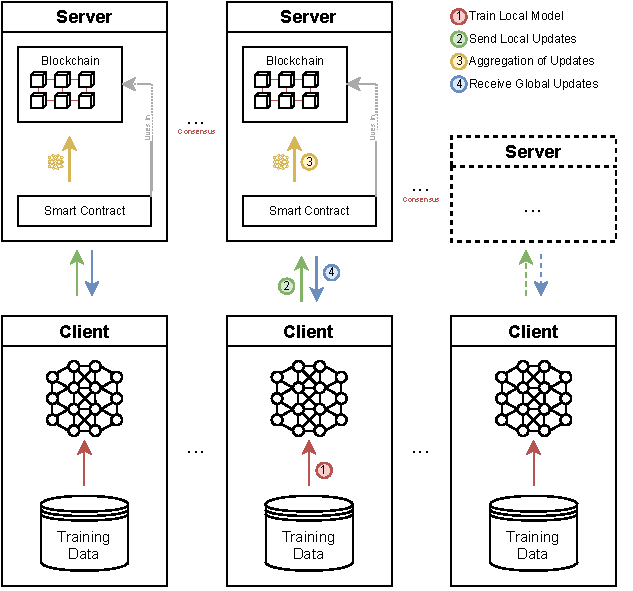
\includegraphics[width=0.6\textwidth]{graphics/bfl-architecture.pdf}
    \caption{Blockchain-based Federated Learning Architecture}
    \label{fig:bfl_arch}
\end{figure}



\subsection{Participants Selection Algorithms}

Participant selection algorithms are algorithms that are used to decide how many and which clients are selected to participate in each round. There are two main participant selection algorithms:

\begin{itemize}
    \item \textit{Random selection}, where both the number of participants, as well as the participants themselves are selected randomly before the start of each round.
    
    \item \textit{First-come first-served}, where the number of participants $n$ is chosen randomly before the start of each round. Then, the first $n$ clients to take initiative to join the round will participate.
\end{itemize}

\subsection{Scoring and Aggregation Algorithms}
\label{background:scoring}

During the training process, each client produces its model parameter updates and communicates them to the servers through the blockchain. These parameters are then aggregated. However, there are different security aspects that should be taken into account here as the parameter updates creates a possibility for performing different attacks such as poisoning attacks \cite{9134967} and plagiarism attacks \cite{10.48550/arxiv.2009.09338}.

\begin{itemize}
    \item \textit{Poisoning attacks} happen when clients willingly send parameter updates that decrease the quality of the model. They may have been generated using an unreliable data set, or done on purpose. To avoid other participants to provide unreliable data to degrade the model performance, there are dynamic verification techniques \cite{10.48550/arxiv.2110.02182, 10.48550/arxiv.2104.10501} that allow to ignore low quality data.
    
    \item \textit{Plagiarism attacks} happen when lazy clients plagiarize other client's models updates without really training their models. These attacks can be addressed via pseudo-noise algorithms \cite{9403374}. In addition, plagiarism attacks within the same round can be avoided by secure communication methods, such as differential privacy \cite{10.48550/arxiv.2009.09338}, through which plagiarism attacks where a client reuses parameters from a previous round can be avoided by simply comparing the different client's updates.
\end{itemize}

To mitigate the poisoning and plagiarism attacks, different scoring algorithms were developed. Scoring algorithms are used to give each client, or its model update, a score. Based on this score, the submission may have more or less impact on the aggregation, if any at all. In addition, scores are used for reward mechanisms in systems where public models are being trained and clients need some sort of incentive to keep participating \cite{8945913, 8832210, 8905038, 9006344}. In this section, we explain briefly how each of the scoring algorithms works and if they influence the aggregation algorithm.

\subsubsection{BlockFlow Score}

The BlockFlow algorithm \cite{10.48550/arxiv.2007.03856} work by giving each submission a score and, based on that score, do the aggregation. In this algorithm, each client $a$ gives each other client $k$ a score $s_{a,k} \in [0.0, 1.0]$, which can be based on $a$'s validation set accuracy using $k$'s submission. Based on this scores, a median score and an evaluation quality scores are calculated. The overall scores will then be the minimum between the scaled median score and the scaled least accurate evaluation score.

With the final scores, the aggregation is calculated using the scores as weights in the Federated Averaging algorithm, instead of the number of samples. More details regarding the algorithm specifics can be found in the original paper.

\subsubsection{Marginal Gain Score}

The Marginal Gain algorithm \cite{10.48550/arxiv.2011.07516}, also known as contributivity score, is calculated by summing the marginal performance gains of all the client's model updates so far. Similarly to BlockFlow scoring, each client has to give each other clients' submission a score. The formula of the client $c$'s submission score $S(c)$ is calculated as follows:

\begin{equation}
    \label{eq:marginal-gain}
    S(c)= \sum_r(v(M_r)-v(M^c_{r+1}))
\end{equation}
, where $v$ is a performance metric, such as accuracy, and $m$ is the model and $r$ the round. These scores are used as weights in the Federated Averaging Algorithm. If the submission's score is equal or below $0$, the submission is ignored.

\subsubsection{Multi-KRUM Score}

The Multi-KRUM algorithm \cite{9170559, Peyvandi2022, 9292450} works by giving each submission a score and eliminating dubious submissions based on their score. This scores are calculated by the servers and are based on the Euclidean distances between the different client $c$'s submissions. The score of each client is denoted as $S(c)$ and calculated as follows:

\begin{equation}
    \label{eq:multi-krum}
    S(c)=\sum_{c \rightarrow k} || \Delta w_c - \Delta w_k|| ^2
\end{equation}

, where $\Delta w$ is a submission and $c \rightarrow k$ are the clients $k$ whose submission $\Delta w_k$ are the $R-f-2$ closest to $\Delta w_c$. In this formula, $R$ is the total number of submissions, while $f$ represents the amount of Byzantine clients. After giving each submission a score, the $R-f$ clients with the lowest scores are chosen and the remaining are rejected. Please note that Byzantine fault tolerant systems behave correctly when no more than $f$ out of $3f+1$ replicas fail.

\subsection{Privacy Mechanisms}

Even though FL is already more secure than centralized ML in the sense that the raw data is never shared, the model weights can be exploited via inference attacks \cite{10.1145/3298981}. Inference attacks are attacks in which the weights are used to reverse-engineer the original data.

Additionally, in BFS systems, the weights are visible to all other client or participant since the blockchain provides an immutable, traceable and auditable record of the whole process. Consequently, it is important to reduce the surface for attacks when it comes to the model parameters.

\subsubsection{(Local) Differential Privacy}\label{background:diff_priv}

Differential Privacy (DP) \cite{hvdiffpriv} is a set of mathematical constrains that algorithms must observe in order to ensure a certain degree of privacy. In other words, some data is differentially private if, by looking at it, we cannot retrieve identifiable information about the original source.

Local Differential Privacy \cite{10.48550/arxiv.2009.09338, 9415623} is a model of Differential Privacy that ensures a specific degree of privacy, usually by using a randomized algorithm $A$ to apply noise to the original data \cite{wei2022vertical}. We say that $A$ provides $\epsilon$-local differential privacy if, and only if, for all subsets $S$ of the image of $A$, and for all pairs of private data $x$ and $x'$:

\begin{equation}
    \label{eq:e-ldp}
    \Pr[A(x) \in S] \leq e^\epsilon \times \Pr[A(x') \in S]
\end{equation}

, where the probability is taken from the randomized algorithm. The lower the $\epsilon$, the higher the degree of privacy.



